\subsubsection{Intelligent Care}

% \begin{wrapfigure}{l}{0.5\textwidth}
%     \centering
%     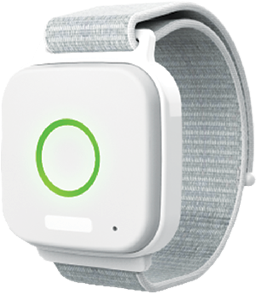
\includegraphics[width=0.5\linewidth]{report//images/intelligent_care.png}
%     \caption{Intelligent Care "Alarmtryk" (\textit{alarm button})}
%     \label{fig:intelligent_care}
% \end{wrapfigure}


Another related product is the Intelligent Care system. Their focus lies more towards nursing homes, assisted living and other institutions, rather than individual use. This is due to its focus around a gateway / hub, that needs constant connection to their cloud. For larger institutions multiple gateways are then needed to cover all the possible areas that a patient or resident might be located in. Their products then work by connecting to, and sending signals to the nearest hub. This is great for zone or room identification as they advertise, but lacks the ability to detect any emergencies outside of the range of the gateways. But what it lacks in range it makes up for in precision, due to the fact that it doesn't rely on \gls{gps} signals indoors, which are notoriously unreliable.

\wrapimage{l}
    {report//images/intelligent_care.png}
    {Intelligent Care "Alarmtryk"}
    {intelligent_care}

The main related product that would solve our problem is their \textit{Alarmtryk (NT-SMID-869-RFID)}, a wristband that allows patients and residents to push a button on their wrist to alert the gateway, and thereby alert the staff. This wristband also acts as an access control device, allowing residents in nursing homes to unlock their own door with their wristband, helping to ensure that the patient remembers to wear it. 
